%%%%%%%%%%%%%%%%%%%%%%%%%%%%%%%%%%%%%%%%%%%%%%%%%%%%%%%%%%%%%%%%%%%%%%%%
%
% Template latex file for a common article class for class notes
% and write ups. Additional Configuration and styling options are 
% commented out. ex. Table of Contents and Title page
% 
% Author: Amy Bui
% 
%%%%%%%%%%%%%%%%%%%%%%%%%%%%%%%%%%%%%%%%%%%%%%%%%%%%%%%%%%%%%%%%%%%%%%%%
 
\documentclass[12pt]{article}
\usepackage[utf8]{inputenc}
\usepackage{parskip}
\usepackage{tabularx}
\usepackage{array}
\usepackage{appendix}
% \usepackage[showframe=true]{geometry}
\usepackage{changepage}
% \usepackage{csvsimple}
% \usepackage[framemethod=tikz]{mdframed}
% \usepackage[color, leftbars]{changebar}
% \usepackage[inkscapeformat=png]{svg}
% \usepackage{svg}
% \usepackage[inkscape={/Applications/Inkscape.app/Contents/Resources/bin/inkscape -z -C}]{svg}

% Important Configurations
 
%%%%%%%%%%%%%%%%%%%%%%%%%%%%%%%%%%%%%%%%%%%%%%%%%%%%%%%%%%%%%%%%%%%%%%%%
% Reduce margin
%
% \addtolength{\oddsidemargin}{-.85in}
% \addtolength{\evensidemargin}{-.85in}
% \addtolength{\textwidth}{1in}

% \addtolength{\topmargin}{-.85in}
% \addtolength{\textheight}{1in}

% Page format commands:
% Override normal article margins,
% making the margins smaller
\setlength{\textwidth}{6.5in}
\setlength{\textheight}{9in}
\setlength{\oddsidemargin}{0in}
\setlength{\evensidemargin}{0in}
\setlength{\topmargin}{-0.6in}

\setlength{\parindent}{0pt}
%%%%%%%%%%%%%%%%%%%%%%%%%%%%%%%%%%%%%%%%%%%%%%%%%%%%%%%%%%%%%%%%%%%%%%%%


%%%%%%%%%%%%%%%%%%%%%%%%%%%%%%%%%%%%%%%%%%%%%%%%%%%%%%%%%%%%%%%%%%%%%%%%
% Math Symbols
\usepackage{mathtools}
\usepackage{amssymb}
% \usepackage{epsfig}
\usepackage{amsmath,amsthm}
\usepackage{amscd,amsxtra,latexsym}


% add floor and ceiling symbol. Usage: \ceil*{}, \floor*{}
\DeclarePairedDelimiter\ceil{\lceil}{\rceil}
\DeclarePairedDelimiter\floor{\lfloor}{\rfloor}

% multiset \langle ... \rangle
\def\multiset#1#2{\ensuremath{\left(\kern-.3em\left(\genfrac{}{}{0pt}{}{#1}{#2}\right)\kern-.3em\right)}}



%%%%%%%%%%%%%%%%%%%%%%%%%%%%%%%%%%%%%%%%%%%%%%%%%%%%%%%%%%%%%%%%%%%%%%%%

%%%%%%%%%%%%%%%%%%%%%%%%%%%%%%%%%%%%%%%%%%%%%%%%%%%%%%%%%%%%%%%%%%%%%%%%
% Code Sample Styling

% use \lstinline! xxx ! or \begin{lstlisting} ... \end{lstlisting}
\usepackage{listings}

\usepackage{color}
\definecolor{light-gray}{gray}{0.97} % shade of grey
\definecolor{dkgreen}{rgb}{0,0.6,0}
\definecolor{gray}{rgb}{0.5,0.5,0.5}
\definecolor{mauve}{rgb}{0.58,0,0.82}

% \begin{lstlisting}[...] ... \end{lstlisting}
\lstset{frame=none,
    language=Verilog,
    aboveskip=3mm,
    belowskip=3mm,
    stepnumber=0, % set to 0 if you don't like line nums
    showstringspaces=false,
    columns=flexible,
    basicstyle={\small\ttfamily},
    numbers=left,
    numberstyle=\color{black},
    keywordstyle=\color{blue},
    commentstyle=\color{dkgreen},
    stringstyle=\color{mauve},
    backgroundcolor=\color{light-gray},
    breaklines=true,
    breakatwhitespace=false,
    tabsize=2
}

% \newcommand\mylstcaption{}

% \mdfdefinestyle{mymdstyle}{
% hidealllines=true,
% middleextra={
%   \node[anchor=west] at (O|-P)
%     {\lstlistingname~\thelstlisting\  (Cont.):~\mylstcaption};},
% secondextra={
%   \node[anchor=west] at (O|-P)
%     {\lstlistingname~\thelstlisting\  (Cont.):~\mylstcaption};},
% splittopskip=2\baselineskip
% }

% \surroundwithmdframed[style=mymdstyle]{lstlisting}
% \newmdenv[style=mymdstyle]{mdlisting}



%%%%%%%%%%%%%%%%%%%%%%%%%%%%%%%%%%%%%%%%%%%%%%%%%%%%%%%%%%%%%%%%%%%%%%%%

%%%%%%%%%%%%%%%%%%%%%%%%%%%%%%%%%%%%%%%%%%%%%%%%%%%%%%%%%%%%%%%%%%%%%%%%
\usepackage{xcolor}
%% https://tex.stackexchange.com/questions/401750/quick-and-short-command-for-coloring-one-word
\newcommand\shorthandon{\catcode`@=\active \catcode`^=\active \catcode`*=\active }
\newcommand\shorthandoff{\catcode`@=12 \catcode`^=7 \catcode`*=12 }
\shorthandon
\def@#1@{\textcolor{red}{#1}}%
\def^#1^{\textcolor{blue}{#1}}%
\def*#1{\string#1}
\shorthandoff
%% useage: \textcolor{red}{text here}
% \shorthandon
% This is a @test@ of the ^emergency^ bro*@dcast system.
% \shorthandoff
%%%%%%%%%%%%%%%%%%%%%%%%%%%%%%%%%%%%%%%%%%%%%%%%%%%%%%%%%%%%%%%%%%%%%%%%


%%%%%%%%%%%%%%%%%%%%%%%%%%%%%%%%%%%%%%%%%%%%%%%%%%%%%%%%%%%%%%%%%%%%%%%%

%Commands below change page margins (this much space at the titlepage, etc)
\newlength{\toppush}
\setlength{\toppush}{2\headheight}
\addtolength{\toppush}{\headsep}

% Section header Styling
% The commands below change the bold text where it says "Section" into "Question"
% \usepackage{titlesec}
% \titleformat{\section}
% {\normalfont\Large\bfseries}{Question~\thesection:}{1em}{}

% I added this command below to chance "subsections numbers" to be "Question [subsection number]" -AB 1/31/2021
% \titleformat{\subsection}
% {\normalfont\bfseries}{\thesubsection:}{1em}{}

% Page head Styling
% Name and subject of the class
\def\subjnum{EE 156}          % Class Number
\def\subjname{Advance Topics in Computer Architecture}       % Class Name

% Name of the student, university name and which semester
\def\doheading#1#2#3{\vfill\eject\vspace*{-\toppush}%
  \vbox{\hbox to\textwidth{{\bf} \subjnum: \subjname \hfil Amy Bui}%
    \hbox to\textwidth{{\bf} Tufts University, Spring 2023 \hfil#3\strut}%
    \hrule}}

%Command for the title of the document (Homework 0)
\newcommand{\htitle}[1]{\vspace*{1.25ex plus 1ex minus 0ex}%
\begin{center}
    {\large\bf #1}
\end{center}} 
%%%%%%%%%%%%%%%%%%%%%%%%%%%%%%%%%%%%%%%%%%%%%%%%%%%%%%%%%%%%%%%%%%%%%%%%



%%%%%%%%%%%%%%%%%%%%%%%%%%%%%%%%%%%%%%%%%%%%%%%%%%%%%%%%%%%%%%%%%%%%%%%%
% Misc
\usepackage{graphicx} % graphics
\usepackage{enumitem} % listing style (bullet lists)

% below helps with trying to get figures in a row
\usepackage{caption}
\usepackage{subcaption}

% hyperlink styling
% use \href{} and \url{}, and colors table of contents links
% use \href{} and \url{}
% \label{sec:name}
% \hyperref[label]{text}
\usepackage{hyperref}
\hypersetup{
    colorlinks=true,
    linkcolor=blue, % was previously black
    filecolor=magenta,
    urlcolor=blue,
    pdftitle={Template}
}
\urlstyle{same}

% A command for primes (')
\newcommand{\p}%
    {\ensuremath{^{\prime}}}

% a command for double primes ('')
\newcommand{\pp}%
    {\ensuremath{^{\prime \prime}}}

% A command for the Kleene star
\newcommand{\str}%
    {\ensuremath{^{\star}}}

% a command for the double star
\newcommand{\sstr}%
    {\ensuremath{^{\star\star}}}
%%%%%%%%%%%%%%%%%%%%%%%%%%%%%%%%%%%%%%%%%%%%%%%%%%%%%%%%%%%%%%%%%%%%%%%%

% Options for title page, use \maketitle in document
% \author{Amy Bui}
% \title{COMP160 - Algorithms: Class Notes and Practice}


\begin{document}
%% create title page
% \title{(g)ROOT \\ Language Reference Manual}
% \author{Samuel Russo \quad Amy Bui \quad Eliza Encherman \\ Zachary Goldstein \quad Nickolas Gravel}
% \date{\today}
% \maketitle

\doheading{2}{title}{Lab 1}

    %%%%%%%%%%%%%%%%%%%%%%%%%%%%%%%%%%%%%%%%%%%%%%%%%%%%%%%%%%%%%%%%%%%%%%%%
    % Table of Contents
    \setcounter{tocdepth}{2}
    \tableofcontents
    % \pagebreak
    %%%%%%%%%%%%%%%%%%%%%%%%%%%%%%%%%%%%%%%%%%%%%%%%%%%%%%%%%%%%%%%%%%%%%%%%

    \begin{thebibliography}{1}
        \bibitem[1]{sniper}\href{https://snipersim.org/w/The_Sniper_Multi-Core_Simulator}{The Sniper Multi-Core Simulator}
        \bibitem[2]{parallel}O. Tange (2011): \href{https://www.gnu.org/software/parallel/parallel_tutorial.html}{GNU Parallel}  - The Command-Line Power Tool
        \bibitem[3]{splash2}S. C. Woo, M. Ohara, E. Torrie, J. P. Singh and A. Gupta, \href{https://citeseerx.ist.psu.edu/viewdoc/download?doi=10.1.1.48.2356&rep=rep1&type=pdf}{The SPLASH-2 Programs: Characterizaion and Methodological Considerations}, Proceedings 22nd Annual International Symposium on Computer Architecture, Santa Margherita Ligure, Italy, 1995, pp. 24-36
        \bibitem[4]{npb}Bailey DH, Barszcz E, Barton JT, et al. \href{https://www.nas.nasa.gov/software/npb.html}{The Nas Parallel Benchmarks}. The International Journal of Supercomputing Applications. 1991;5(3):63-73. doi:\url{10.1177/109434209100500306}
        \bibitem[5]{book}John L. Hennessy and David A. Patterson. 2017. Computer Architecture, Sixth Edition: A Quantitative Approach (6th. ed.). Morgan Kaufmann Publishers Inc., San Francisco, CA, USA.
        \bibitem[6]{parallelenergy}S. M. Londono and J. P. de Gyvez, "Extending Amdahl's law for energy-efficiency," 2010 International Conference on Energy Aware Computing, Cairo, Egypt, 2010, pp. 1-4, doi: 10.1109/ICEAC.2010.5702300.
        \bibitem[7]{lab0}Bui, Amy. EE156 Lab0 Report. 2023.
    \end{thebibliography}
    \clearpage

    \section{Intro}
    \label{intro}
    % \clearpage
    %%%%%%%%%%%%%%%%%%%%%%%%%%%%%%%%%%%%%%%%%%%%%%%%%%%%%%%%%%%%%%%%%%%%%%%%
    

    \section{Experimental Setup}
    \label{sec:setup}
        \begin{table}
        \begin{center} 
            \begin{tabular}{c||c||c}
                \begin{tabular}{|l|}
                    \hline
                    \textbf{Benchmark} \\ 
                    \hline 
                    \hline
                    \texttt{splash2-ocean.cont} \\ 
                    \texttt{splash2-radix}\\
                    \texttt{npb-is}\\
                    \hline 
                \end{tabular}
                & 
                \begin{tabular}{|l|}
                    \hline
                    \textbf{L3 Associativity} \\ 
                    \hline 
                    \hline
                    8 \\ 
                    16 \\
                    32 \\
                    \hline 
                \end{tabular}
                &
                \begin{tabular}{|l|}
                    \hline
                    \textbf{L3 Eviction Policy} \\ 
                    \hline 
                    \hline
                    \texttt{LRU} \\ 
                    \texttt{SRRIP}\\
                    \texttt{Round Robin}\\
                    \hline 
                \end{tabular}
            \end{tabular}
            \caption{Configuration parameters and values swept in the experiment.}
            \label{table:configurations}
        \end{center}
        \end{table}

        Simulations ran for an x86 architecture simulator, Sniper 7.3 \cite{sniper}. Each were configured with 4 cores and the same L1, L2, and L3 cache sizes (64 KB, 128 KB, and 512 KB, respectively, each using 64 byte blocks); remaining relevant configuration values were set in the \texttt{gainestown.cfg}. Input size used for all tests was preset \texttt{large}. Figure \ref{topology} visualizes the topologies for all simulations since cache sizes remained constant. 

        Three different L3 cache associativities, three different L3 replacement policies, and three benchmarks were swept in this experiment, for a total of 27 simulations (see Table \ref{table:configurations}). L3 is the largest and slowest cached memory unit compared to L1 and L2; it is also shared across the four cores, while each core has their own L1 and L2 caches. Therefore, we picked the lowest performing cache level used by the processing unit to sweep because it is likely to have common impact on performance and energy that is observable on all four cores. The different configurations were simulated with two \texttt{splash2} benchmarks (\texttt{ocean.cont} and \texttt{radix} \cite{splash2}) and one NAS parallel benchmark (\texttt{npb}) (\texttt{is} \cite{npb}). The workloads are briefly described as follow:

        \begin{description}
            \item[\textbf{splash2-ocean.cont}]: The \texttt{ocean} suite of test studies large-scale ocean movements based on currents, and uses 4D array grids and a red-black Gauss-Seidel multigrid equation solver. 
            \item[\textbf{splash2-radix}]: The \texttt{radix} suite uses an iterative radix sort algorithm that generates histograms and has each processor permute array index keys, a process that depends on processors communicating in order to determine keys thorough writes.
            \item[\textbf{npb-is}]: The NASA Advanced Supercomputing (NAS) Parallel Benchmarks (NPB) are a set of benchmarks tuned for highly parallel workloads. The \texttt{is} kernal performs a sorting operation that is important as ``particle method'' code (ex. simulations of mechanics (solid, fluid, etc.) as discrete ``particles''), testing both integer computation speed and communication performance. This benchmark excludes floating point arithmetic. 
        \end{description}

        Three varied replacement policies were chosen in order to observe the effects of different replacement models on power and performance. They are as follow:
        \begin{description}
            \item[\textbf{Least Recently Used (LRU)}]: LRU is a recency-based policy that replaces the least recently used block, which involved tracking when blocks are accessed/re-referenced.
            \item[\textbf{Static Re-Reference Interval Prediction (SRRIP)}]: SRRIP is a policy that uses a re-reference prediction value (RRPV) to ``predict'' the how likely a block will be referenced again; this policy uses 2-bit RRPV and is likely to evict recently inserted cache blocks. 
            \item[\textbf{Round Robin}]: Round robin is a queue-based policy that replaces the cache blocks in sequential order, evicting the oldest block in a set in a first-in-first-out (FIFO) manner.
        \end{description}
        

        Simulations had either 8-, 16-, or 32-way L3 set associativity in order to observe how power and performance changed with the number of ways. L1 and L2 caches remained 4- and 8-way set associative, respectively, and both used LRU by default. SniperSim McPAT could not output data for a 64-way set associativity for the given L3 cache size (512 KB) and block size (64 bytes) and so was excluded from the experiment. 

        All the simulations ran concurrently using bash script(s) and GNU \texttt{parallel} shell tool \cite{parallel}, and post processing of the data were handled with python (v2.7) and bash scripts (included separately). Simulations ran on a python virtual environment and in a detached \texttt{tmux} session, due to long duration of the experiments. Sniper provided data processing tools used were: \texttt{gen\_topology.py}, \texttt{cpi-stack.py}, and \texttt{mcpat.py}. 
        
        % TOPOLOGY
        % \begin{figure}[hbt!] 
        %     \centering
        %     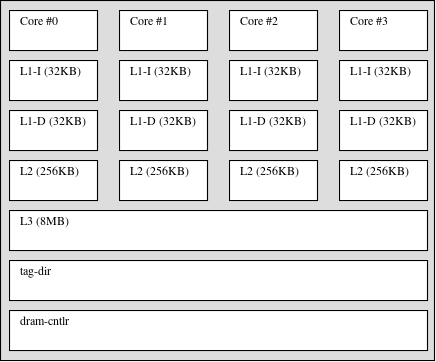
\includegraphics[width=0.5\textwidth]{output/npb-is/8way-lru/topo.png}
        %     \caption{Topology for \texttt{npb-is}, \texttt{splash2-ocean.cont}, and \texttt{splash2-radix} benchmark tests with all consistent cache sizes: 32 KB L1, 128 KS L2, and 512 KB L3. All benchmarks were run in \texttt{Sniper-7.3} with the \texttt{gainestown} configuration using the \texttt{--viz} and \texttt{--roi} options.}
        %     \label{topology} 
        % \end{figure}

    % \clearpage
    %%%%%%%%%%%%%%%%%%%%%%%%%%%%%%%%%%%%%%%%%%%%%%%%%%%%%%%%%%%%%%%%%%%%%%%%

    \section{Results \& Analysis}
    % \clearpage
    %%%%%%%%%%%%%%%%%%%%%%%%%%%%%%%%%%%%%%%%%%%%%%%%%%%%%%%%%%%%%%%%%%%%%%%%


    \section{Conclusion}
    \label{conclusion}
    % \clearpage
    %%%%%%%%%%%%%%%%%%%%%%%%%%%%%%%%%%%%%%%%%%%%%%%%%%%%%%%%%%%%%%%%%%%%%%%%

    \section{Appendix: Raw Post Processed Data}
    \label{appendix:raw}

    \subsection{benchmark} %%%%%%%%%%%%%%%%%%%%%%%%%%%%%%%%%%%
        
        \subsubsection{Power Results} %%%%%%%%%%%%%%%%%%%%%%%%%%%%%%%%%%%

        % Power
        % \begin{figure}[hbt!]
        %     \centering 
        %     \begin{adjustwidth}{-2.75cm}{}
        %     \begin{tabular}{ccc}
        %         \begin{subfigure}{0.42\textwidth}
        %             \centering
        %             \includegraphics[width=1\textwidth]{output/npb-is/8way-lru/power-chop.png}
        %             \caption{L3 energy 0.20 J; Total energy 16.79 J}
        %             \label{appfig:power:is:lru:8}
        %         \end{subfigure} &
        %         \begin{subfigure}{0.42\textwidth}
        %             \centering
        %             \includegraphics[width=1\textwidth]{output/npb-is/16way-lru/power-chop.png}
        %             \caption{L3 energy 0.21 J; Total energy 16.43 J}
        %             \label{appfig:power:is:lru:16}
        %         \end{subfigure} &
        %         \begin{subfigure}{0.42\textwidth}
        %             \centering
        %             \includegraphics[width=1\textwidth]{output/npb-is/32way-lru/power-chop.png}
        %             \caption{L3 energy 0.27 J; Total energy 16.40 J}
        %             \label{appfig:power:is:lru:32}
        %         \end{subfigure} 
        %     \end{tabular}
        %     \end{adjustwidth}
        %     \caption{Processor power with an (\ref{appfig:power:is:lru:8}) 8-way, (\ref{appfig:power:is:lru:16}) 16-way, and (\ref{appfig:power:is:lru:32}) 32-way L3 cache using LRU replacement policy.}
        %     \label{appfig:power:is:lru}
        % \end{figure}

        % legend
        % \begin{figure}
        %     \centering 
        %     \begin{adjustwidth}{-2.75cm}{}
        %     \begin{tabular}{ccc}
        %         & & 
        %         \begin{subfigure}{0.33\textwidth}
        %             \centering
        %             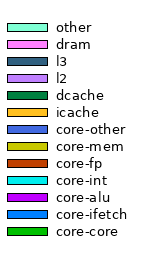
\includegraphics[width=1\textwidth]{output/npb-is/8way-lru/power-legend.png}
        %             % \caption{}
        %             \label{appfig:power:is:legend}
        %         \end{subfigure} 
        %     \end{tabular}
        % \end{adjustwidth}
        % \end{figure}
        % \clearpage

        % \begin{figure}[hbt!]
        %     \centering
        %     \noindent\begin{subfigure}{0.75\textwidth}
        %     \lstinputlisting{output/npb-is/8way-lru/power.out}
        %     \caption{}
        %     \end{subfigure}%

        %     \noindent\begin{subfigure}{0.75\textwidth}
        %     \lstinputlisting{output/npb-is/16way-lru/power.out}
        %     \caption{}
        %     \end{subfigure}%
        % \end{figure}
        % \clearpage

        % \begin{figure}[hbt!]\ContinuedFloat
        %     \centering
        %     \noindent\begin{subfigure}{0.75\textwidth}
        %     \lstinputlisting{output/npb-is/32way-lru/power.out}
        %     \caption{}
        %     \end{subfigure}%
        %     \caption{Specific values for each components' power consumption (See. Fig. \ref{appfig:power:is:lru}), for \texttt{npb-is} benchmark with (LRU) L3 associativity of (a) 8, (b) 16, and (c) 32 way.}
        %     \label{appfig:power:is:lru:values}
        % \end{figure}
        % \clearpage

        %%%%%%%%%%%%%%%%%%%%%%%%%%%%%%%%%%%%%%%%%%%%%%%%%%%%%%%%%%%%%%%%%%%%%%

        \subsubsection{CPI Stacks} %%%%%%%%%%%%%%%%%%%%%%%%%%%%%%%%%%%

        % CPI Result
        % \begin{figure}[hbt!]
        %     \centering 
        %     \begin{adjustwidth}{-2.75cm}{}
        %     \begin{tabular}{ccc}
        %         \begin{subfigure}{0.42\textwidth}
        %             \centering
        %             \includegraphics[width=1\textwidth]{output/npb-is/8way-lru/cpi-stack-chop.png}
        %             \caption{}
        %             \label{appfig:cpi:is:lru:8}
        %         \end{subfigure} &
        %         \begin{subfigure}{0.42\textwidth}
        %             \centering
        %             \includegraphics[width=1\textwidth]{output/npb-is/16way-lru/cpi-stack-chop.png}
        %             \caption{}
        %             \label{appfig:cpi:is:lru:16}
        %         \end{subfigure} &
        %         \begin{subfigure}{0.42\textwidth}
        %             \centering
        %             \includegraphics[width=1\textwidth]{output/npb-is/32way-lru/cpi-stack-chop.png}
        %             \caption{}
        %             \label{appfig:cpi:is:lru:32}
        %         \end{subfigure} 
        %     \end{tabular}
        %     \end{adjustwidth}
        %     \caption{CPI stack with an (\ref{appfig:cpi:is:lru:8}) 8-way, (\ref{appfig:cpi:is:lru:16}) 16-way, and (\ref{appfig:cpi:is:lru:32}) 32-way L3 cache using LRU replacement policy.}
        %     \label{appfig:cpi:is:lru}
        % \end{figure}

        % legend
        % \begin{figure}
        %     \centering 
        %     \begin{adjustwidth}{-2.75cm}{}
        %     \begin{tabular}{ccc}
        %         & 
        %         \begin{subfigure}{0.33\textwidth}
        %             \centering
        %             \includegraphics[width=1\textwidth]{output/npb-is/32way-rr/cpi-stack-legend.png}
        %             % \caption{}
        %             \label{appfig:cpi:is:legend1}
        %         \end{subfigure} 
        %         & 
        %         \begin{subfigure}{0.33\textwidth}
        %             \centering
        %             \includegraphics[width=1\textwidth]{output/npb-is/16way-srrip/cpi-stack-legend.png}
        %             % \caption{}
        %             \label{appfig:cpi:is:legend2}
        %         \end{subfigure} 
        %     \end{tabular}
        % \end{adjustwidth}
        % \end{figure}

        % Output Values
        % \begin{figure}[hbt!]
        %     \centering
        %     \noindent\begin{subfigure}{0.75\textwidth}
        %     \lstinputlisting{output/npb-is/8way-lru/cpi-stack.out}
        %     \caption{}
        %     \end{subfigure}%

        %     \noindent\begin{subfigure}{0.75\textwidth}
        %     \lstinputlisting{output/npb-is/16way-lru/cpi-stack.out}
        %     \caption{}
        %     \end{subfigure}%
        % % \end{figure}
        % % \clearpage

        % % \begin{figure}[hbt!]\ContinuedFloat
        % %     \centering
        %     \noindent\begin{subfigure}{0.75\textwidth}
        %     \lstinputlisting{output/npb-is/32way-lru/cpi-stack.out}
        %     \caption{}
        %     \end{subfigure}%
        %     \caption{Specific values for each components' CPI stack fraction of time (See. Fig. \ref{appfig:cpi:is:lru}), for \texttt{npb-is} benchmark with (LRU) L3 associativity of (a) 8, (b) 16, and (c) 32 way.}
        %     \label{appfig:cpi:is:lru:values}
        % \end{figure}
    % \clearpage
   %%%%%%%%%%%%%%%%%%%%%%%%%%%%%%%%%%%%%%%%%%%%%%%%%%%%%%%%%%%%%%%%%%%%%%

\end{document}